\section{Theoretical Background} \label{sec:theory}
The purpose of this chapter is to go through the preliminary wind turbine (WT) theory. (Subject to change!)

\subsection{Aerodynamics and airfoil theory} \label{sec:theory_aero}
The sun delivers energy to the earth by heating up the surface and subsequently the air of the earth. Winds occur as a result of the pressure differences that occur due to the expansion and contraction of the air. 

WTs work because they are able to convert the wind's energy into a torque in the generator which then generates electrical energy. When the wind blows over the blades of a WT it delivers some of its energy to the blade, yielding both a thrust force and torque to the blade.

In the simplest 1D momentum theory case the delivery of energy just results in a lowing of the wind speed following the rotor area. Due to mass preservation an expansion would subsequently occur as depicted in \cref{fig:betz}.
\begin{figure}[h]
	\centering
	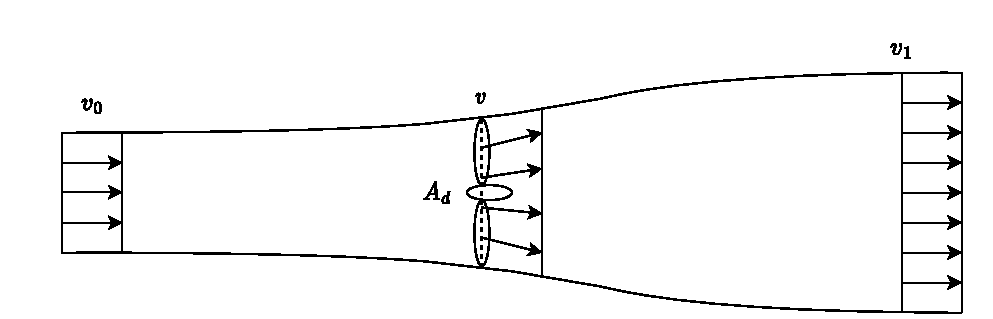
\includegraphics[width=0.8\linewidth]{Graphics/FlowThroughRotor.pdf}
	\caption{Illustration of how the wind in a control volume (CV) changes volume due to its reduction of speed}
	\label{fig:betz}
\end{figure}
The power of the \textit{free} wind $ v_0 $ can be expressed from the wind mass flow $ \dot{m} $ through a control volume:
\begin{equation} \label{eq:power}
	P = \dfrac{1}{2} \dot{m} v_0^2
\end{equation}
The flow of mass can be expressed from the air density $ \rho $, the cross sectional area $ A_d $ of the CV  at the rotor and the free wind speed $ v_0 $ as such:
\begin{equation}\label{eq:mass_deriv}
	\dot{m} = \rho A_d v_0
\end{equation}
Combining \cref{eq:power} and \cref{eq:mass_deriv} yields:
\begin{equation}\label{eq:power2}
	P_{air} = \dfrac{1}{2} \rho A_d v_0^3
\end{equation}
A \textit{power coefficient} $ C_p $ represents the percentage of the available power that is extracted from the wind:
\begin{equation}\label{eq:power_w_Cp}
	P_{T} = \dfrac{1}{2} \rho A_d v_0^3 C_p
\end{equation}
$ C_p $ is dependent on the rotor blade pitch $ \theta $ and the tip speed ratio (TSR) $ \lambda $. In the partial load region the goal is to reach a maximum $ C_p $ by adjusting $ \theta $ and  $ \lambda $ to their optimal values:
\begin{equation}\label{eq:cp_optimal}
	C_p^\star = C_p(\theta^\star, \lambda^\star)
\end{equation}
The TSR is the ratio between the speed of the tip of the WT blade $ (\Omega R) $ where $ R $ is the distance from the center of the rotor and the blade tip and the incoming free wind $v_0$:
\begin{equation}\label{eq:tipspeedratio}
	\lambda = \dfrac{\Omega R}{v_0}
\end{equation}

The achievable size of $ C_p^\star $ is a matter of the WT design. The \textit{Betz limit} is the highest, optimal $ C_p $ that can be theoretically achieved and can be calculated to be:
\begin{equation}\label{eq:betzlimit}
	C_{pbetz} = 0.5962
\end{equation}
%Most often $ C_p $ is also the measure of efficiency for a WT, but a more intuitive efficiency is  calculate measure efficiency from the Betz limit extractable power:
%\begin{equation}\label{eq:efficiency}
%	\eta = \dfrac{C_p}{C_{pbetz}}
%\end{equation}

%When the air travels over the WT blade the air travels slower on one side than the other as illustrated in \cref{fig:airfoil}. Due to mass conservation the air which moves slower on the underside of the blade expands, creating a higher pressure. Likewise the air moving faster on the upper upper side contracts creating in a lower pressure. Resultingly the blade moves upwards.
%\begin{figure}[h]
%	\centering
%	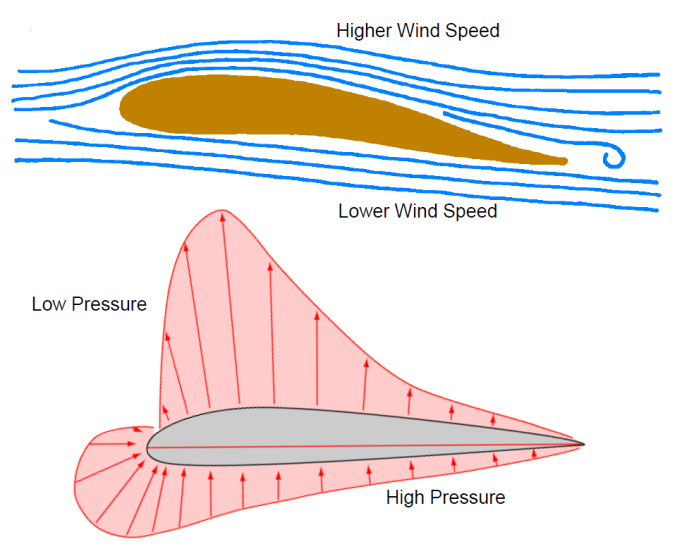
\includegraphics[width=0.5\linewidth]{Graphics/AirfoilAirflow.png}
%	\caption{Illustration of the wind speed difference between the two sides of a WT blade along with an illustration of the induced pressure difference. The result is a lifting force one the blade.}
%	\label{fig:airfoil}
%\end{figure}

Blade element momentum theory is often used to model the forces acting along WT blades. Blade element theory involves breaking a blade into small sections and determining the forces acting on each small section. In \cref{fig:blade_vel_triangle} a cross section of a WT blade can be seen. In this figure, as it is also illustrated at the rotor blade in \cref{fig:betz}, the wind velocity that hits the rotor blades is lowered indicated by the \textit{axial induction factor} $ a $. What is not observed in \cref{fig:betz} is that some of the energy of the wind also goes into driving an airstream around the back of the rotors in the opposite direction of the blade rotation, indicated by the \textit{tangential induction factor} $ a' $. This is known as \textit{swirl losses}.
\begin{figure*}[h]
	\centering
	\subfloat[Blade cross section]{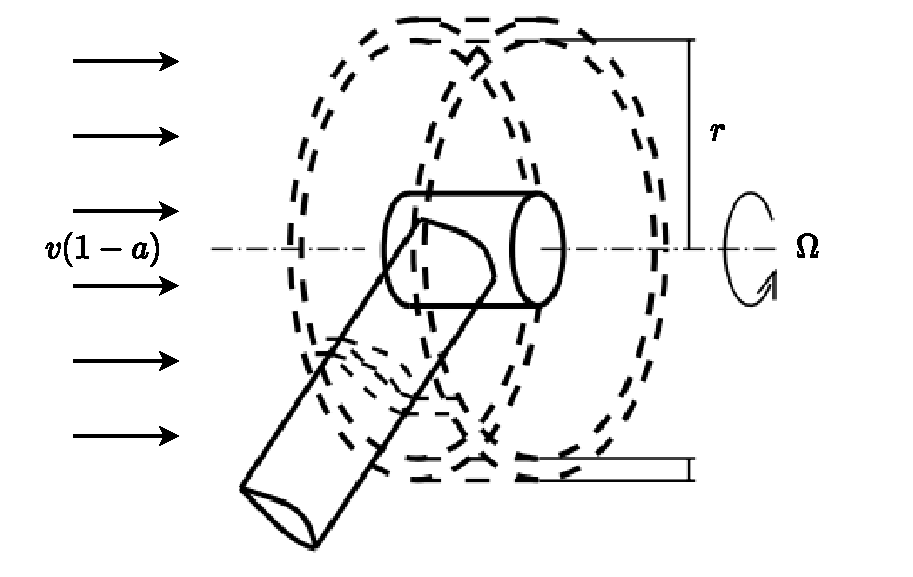
\includegraphics[width=.44\textwidth]{Graphics/RotorBladeElement.pdf}%
		\label{fig:blade_vel_triangles}}
	\hfil
	\subfloat[Velocity triangle]{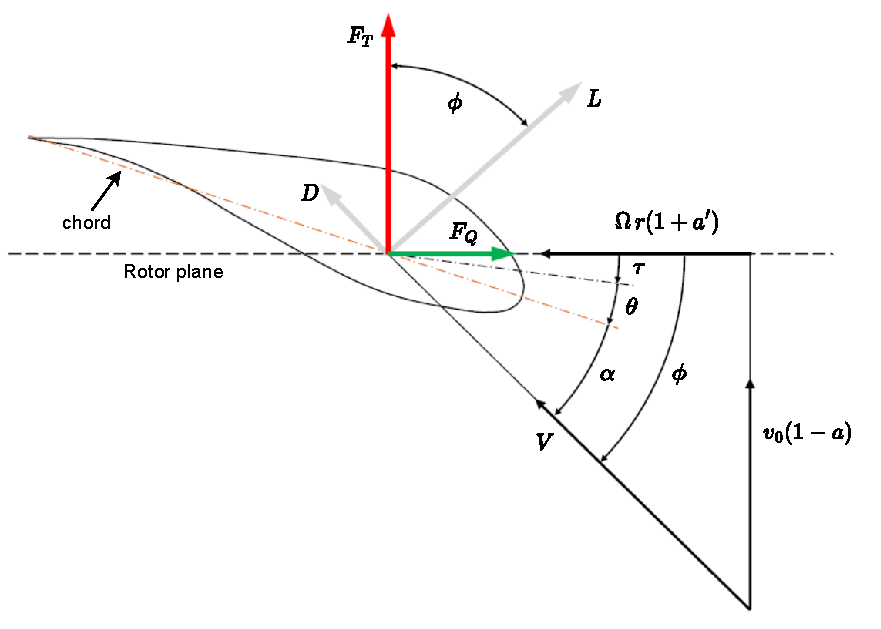
\includegraphics[width=.55\textwidth]{Graphics/BladeVelocityTriangle.pdf}%
		\label{fig:blade_vel_triangle}}
	\caption{Illustrations of a blade cross section and a velocity triangle on a blade section; \textbf{(a)} the blade cross section is made at some distance $ r $ from rotor center and rotates at a frequency $ \Omega $; \textbf{(b)} the velocity triangle acting on a cross section of a WT blade}
	\label{fig:blade_triangles}
\end{figure*}
The resulting air speed is V with an \textit{inflow angle} $ \phi $. $ F_L $ and $ F_D $ are the lift and drag forces on the blade element respectively. They are calculated from \cref{eq:lift} and \cref{eq:drag}. They include the \textit{chord length} $ c $ which is the length from the leading to the trailing edge of the blade.
\begin{align}
	F_L &= \dfrac{1}{2}\,  \rho \, V^2 c \, C_L \label{eq:lift}\\
	F_D &= \dfrac{1}{2} \, \rho \, V^2 c \, C_D \label{eq:drag}
\end{align}
The lift and drag coefficients $ C_L $ and $ C_D $ are usually extracted from table lookups which are typically found from simulations such as Xfoil
\todo{Hvad bruger Vestas til at finde $ C_L $ og $ C_D $?}. 
In a typical scenario $ C_L $ and $ C_D $ are found from the angle of attack $ \alpha $. The thrust and torque vectors $ F_T $ and $ F_Q $ are then calculated from the Pythagorean theorem as in \cref{eq:thrust} and \cref{eq:torque}
%\lipsum[11]\unsure{Is this correct?}\unsure{I'm unsure about also!}
\begin{align}\
	F_T &= L \, cos(\phi) + D \, sin(\phi) \label{eq:thrust} \\
	F_Q &= L \, sin(\phi) - D \, cos(\phi) \label{eq:torque}
\end{align}
The total thrust and torque of a blade can then be calculated by integrating the above over the length of the rotor blade \cite{Knudsen2013}.


\subsection{Wind turbine control} \label{sec:theory_ctrl}
This section includes a walk through of the main functionality of WT control. The standard WT control scheme is explained with regards to different operation regions. Furthermore the challenges presented in FOWT control are examined and some known solutions to the floating control problem are presented. 

\subsubsection{Control regions} \label{sec:theyry_ctrl_regions}
Wind turbine control is split into two main stages of control called partial load control (PLC) and full load control (FLC). In a modern variable-speed-variable-pitch (VPVP) WT such as the one at hind in this project the PLC can be split into three subregions leaving a total of four operating regions. PLC is related to wind speed between cut-in wind speed and rated wind speed. In all three PLC regions the generator power reference is regulated with a PI controller based on a generator speed setpoint to achieve the most optimal power output. The FLC region is related to above rated wind speed to cut-out wind speed. In this region the pitch angle reference is regulated based on a generator speed set-point which is set such that a constant power output is tracked. Furthermore each of the four regions are associated with a specific wind speed range. A visualization of these operating regions can be found in figure \cref{fig:operating_regions}. The figure is simply illustrative and especially the width of the regions are out of proportion. 
\begin{figure}[h]
	\centering
	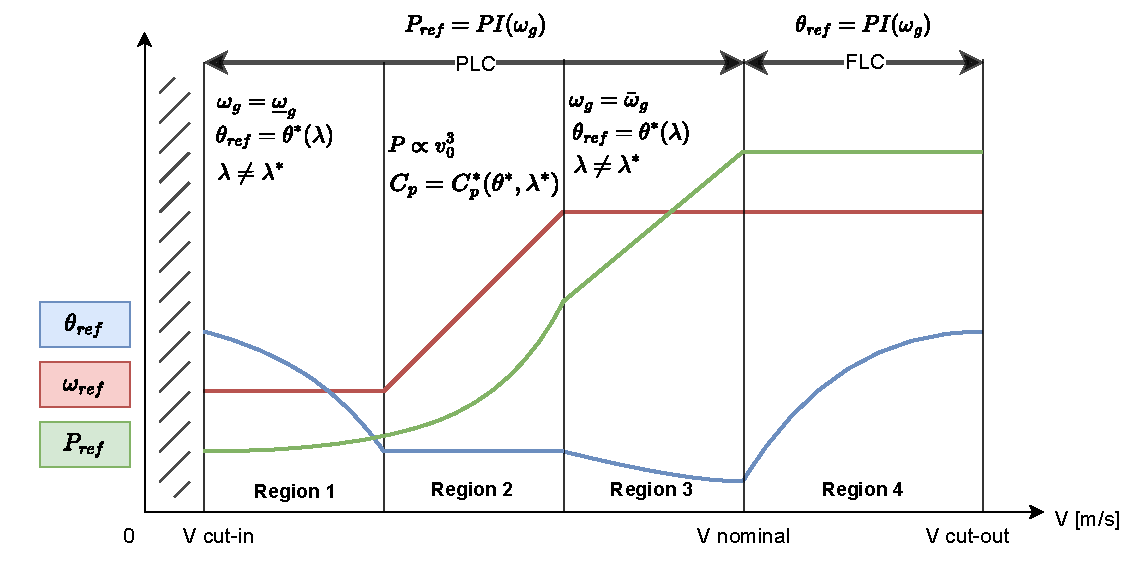
\includegraphics[width=0.9\linewidth]{Graphics/OperatingRegions.pdf}
	\caption{A visualisation of the wind turbine control operating regions. Specific wind speeds are purposefully not included since these are turbine specific. The figure is illustrative and not correctly scaled.}
	\label{fig:operating_regions}
\end{figure}
Below is a short description of the four regions focused on the parameters which are relevant to the control objective which is firstly maximisation of the turbine power output (PLC) and secondly limitation of the power output to nominal power (FLC)
\begin{itemize}
	\item In \textbf{Region 1} the pitch angle reference is set to the optimal angle based on the tip speed ratio which in this region is \underline{not} optimal, meaning that $ C_p \neq C_p^* $. The generator power is set by the PLC PI controller to whatever achieves the minimum rotor speed.
	\item In \textbf{Region 2} the pitch angle reference is set to the optimal angle based on the wind speed. The tip speed ratio is optimal based on the generator speed which is controlled to the optimal value by means of the generator power. The rotor speed is proportional to the wind speed. The power output of the turbine is proportional to the third power of the wind speed. This makes sense in relation to \cref{eq:power_w_Cp}.
	\item In \textbf{Region 3} like in region 1 the angle is set to the optimal angle based on the tip speed which is not optimal. The generator power is set by the PI controller to whatever achieves the maximum allowed rotor speed. The power output of the turbine increases proportional to the wind speed.
	\item In \textbf{Region 4} the pitch angle reference is no longer set at an optimal value. It is now set by the FLC PI controller which tracks a constant nominal power output reference. In FLC the power output and rotor speed is ideally close to constant while the pitch angle changes to counteract changes in turbulence.
\end{itemize}

\begin{figure}[h]
	\centering
	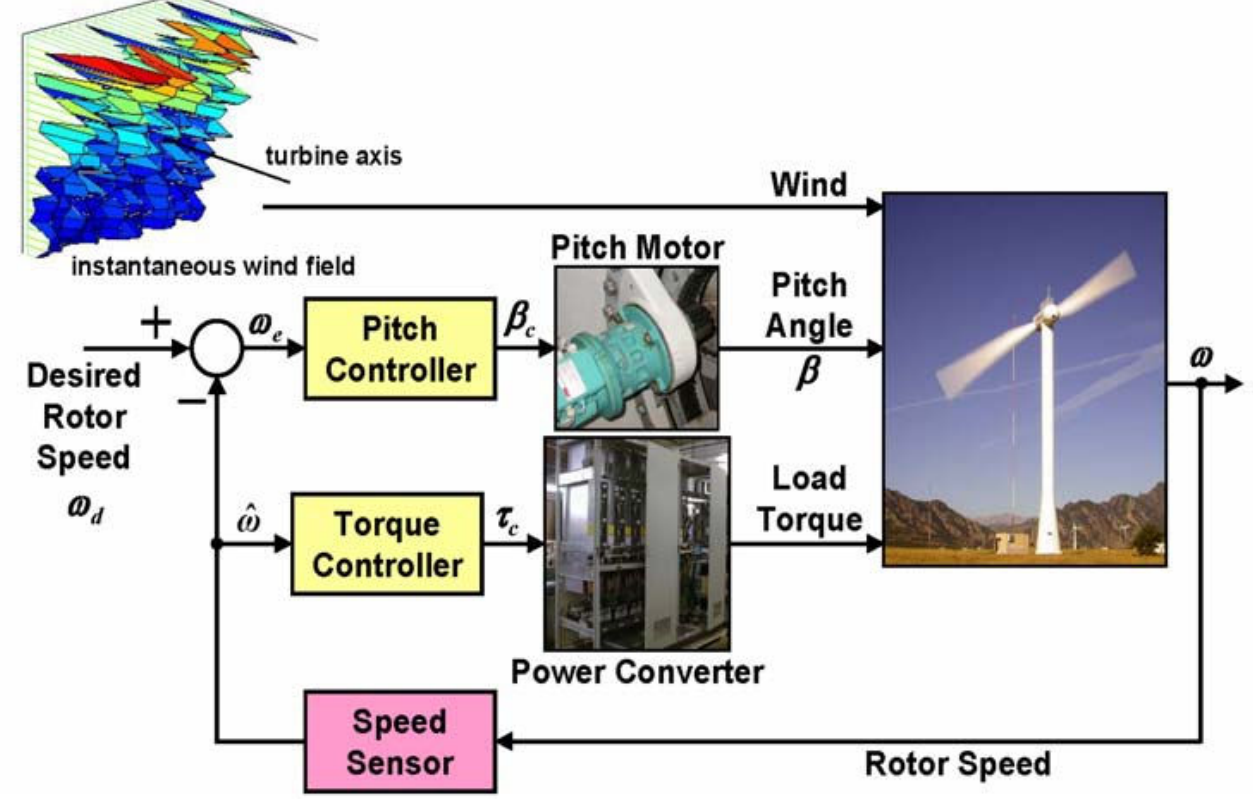
\includegraphics[width=0.7\linewidth]{Graphics/GraphicalWtController.PNG}
	\caption{An overview of the controllers. Figure from \cite{Pao2009}}
	\label{fig:controller_overview}
\end{figure}

\subsubsection{PLC}
In partial load control 

- Cut in -> Nominal
- Power output maximation from C\_P maximation (C\_p\_max)
	- Pitch angle sat at optimal value. Rotor speed regulated to optain optimal omega
- Classic region 2 controller: Torque controller t\_g = KOmega\^2.
- Lower rotor speed limit sat on region 1 to stay clear of 1P and 3P frequencies. GET A DAMN PLOT!!


\todo[inline]{Indsæt figur af CP(theta, omega)!)}


\medskip
\medskip
\medskip
\medskip




\begin{enumerate}
	\item The different stages of control depending on wind speed
	\item \begin{itemize}
		\item 
		\end{itemize}
	\item Full PLC explanation
	\item FUll FLC explanation
	\item FATD - fixed-bottom and floating
\end{enumerate}

\subsubsection{FOWT challenges}
This section concerns the challenges that are persistent in FOWT design and control.



A challenge that both fixed-bottom and FOWT has to deal with is frequency separation with regards to the operating frequencies of the turbine and the periodic disturbances and exciting forces that affect the turbine. Wind and waves will excite the tower at specific frequencies and it is important that such frequencies do not overlap with the turbine modes. Turbine towers are flexible and can as such oscillate. If a disturbance such as waves or the wind excite the WT at the same frequency as the natural frequency of the tower it will cause the tower to oscillate resulting in an increase in fatigue loads. Therefore towers are designed such that their first and second modes do not overlap with especially the 1P and 3P frequencies. 1P is the rotor rotational frequency and 3P is the third multiple of 1P corresponding to the three blades of conventional horizontal WTs.

Vibrations in structures are activated by dynamic periodic forces - like wind, people, traffic and rotating machinery

\begin{itemize}
	\item \textbf{1P} oscillations are typically activated by the periodic force acting on the WT due to the rotor and generator torque.
	\item \textbf{3P} oscillations are typically activated by wind streams going through the rotor plane which strike the rotor blades every time they pass which intuitively is three times for every full rotor rotation.
\end{itemize}
Modern WT towers with a \textit{soft-stiff} tower design are designed such that their first eigenfrequency ends up between the 1P and 3P frequencies and the second eigenfrequency ends up above the 3P frequency. Naturally due to varying rotational frequency both 1P and 3P cover a range of frequencies as illustrated in \cref{fig:1p_and3p}. In the diagram the natural frequency of FOWTs can be observed in frequencies way lower than 1P. The dotted line resembles the location of the second tower mode. In \cref{fig:eigen_and_1p3p} an illustration of the tower modes of both fixed-bottom and floating WTs is found. It is apparent that the first tower mode in a conventional fixed-bottom turbine is due to the flexion of the tower while in the floating structure it is due to the tilting of the whole turbine structure.

\todo[]{Måske også inkludere Campbell diagrammet? Måske bliver det for mange figurer?}



\begin{figure}[h]
	\centering
	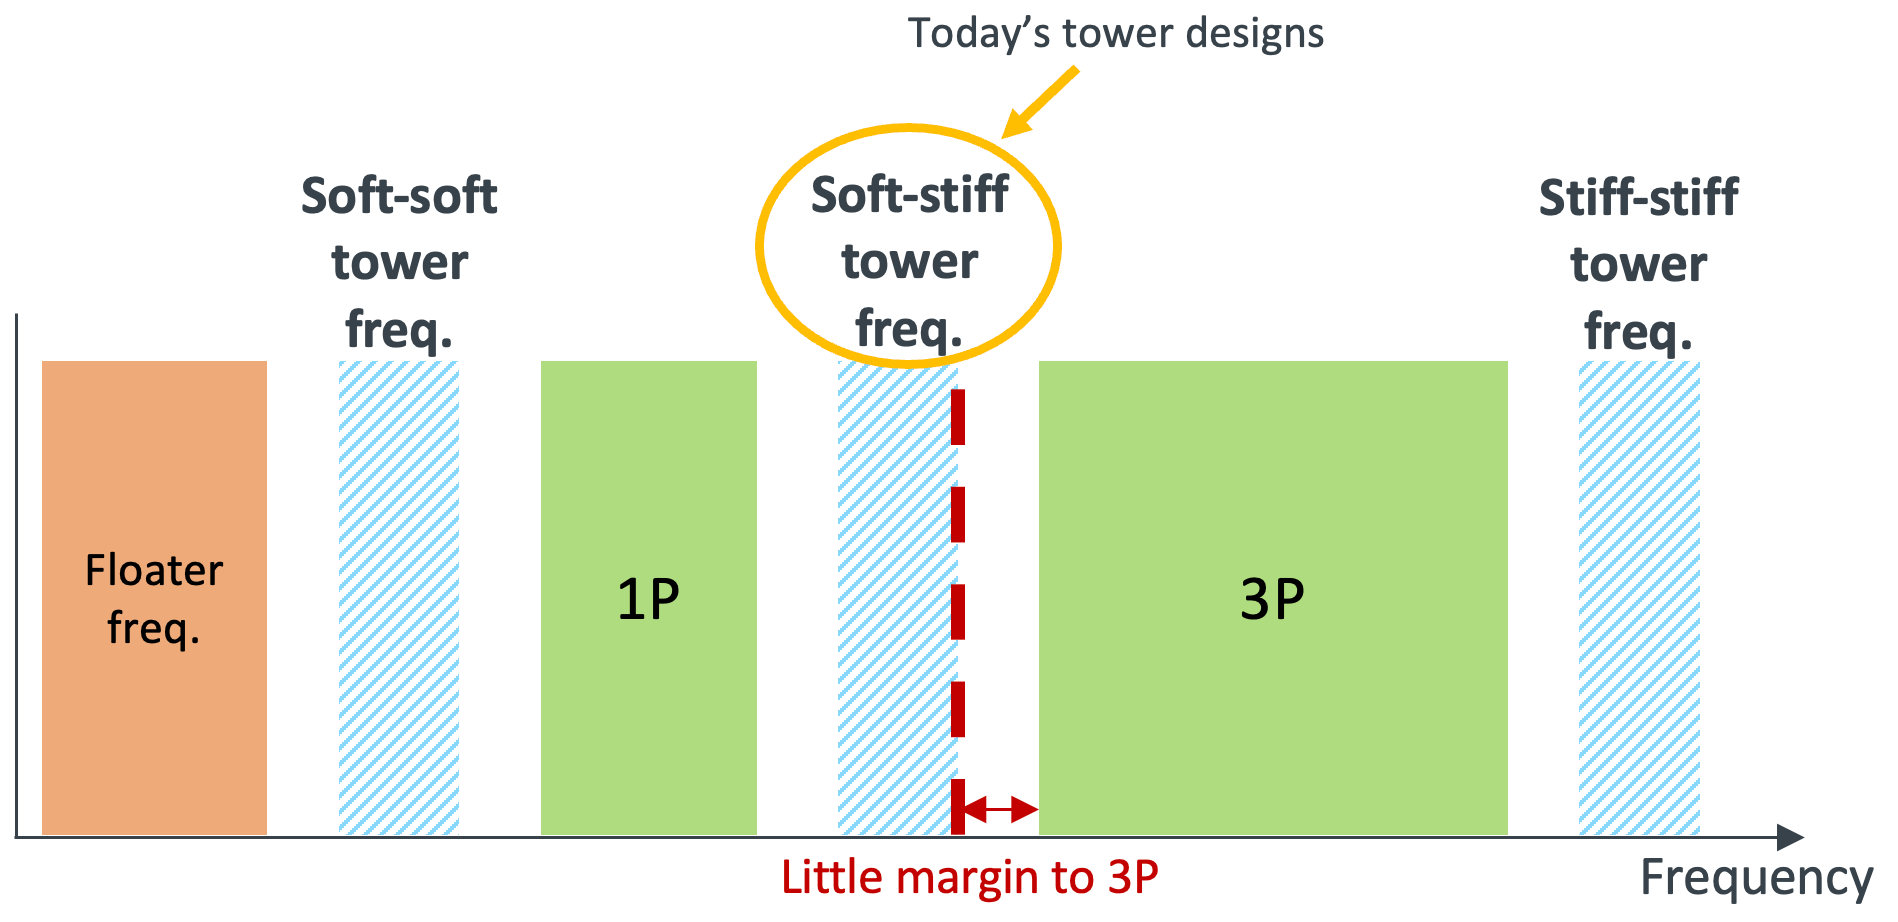
\includegraphics[width=0.7\linewidth]{Graphics/1Pand3PvsTwrStiff.PNG}
	\caption{Illustration of the frequency spans of the tower modes with different designs and for floaters as well as 1P and 3P.}
	\label{fig:1p_and3p}
\end{figure}

In \cref{fig:eigen_and_1p3p} an illustration of the first and second tower mode is found. 


\begin{figure}[h]
	\centering
	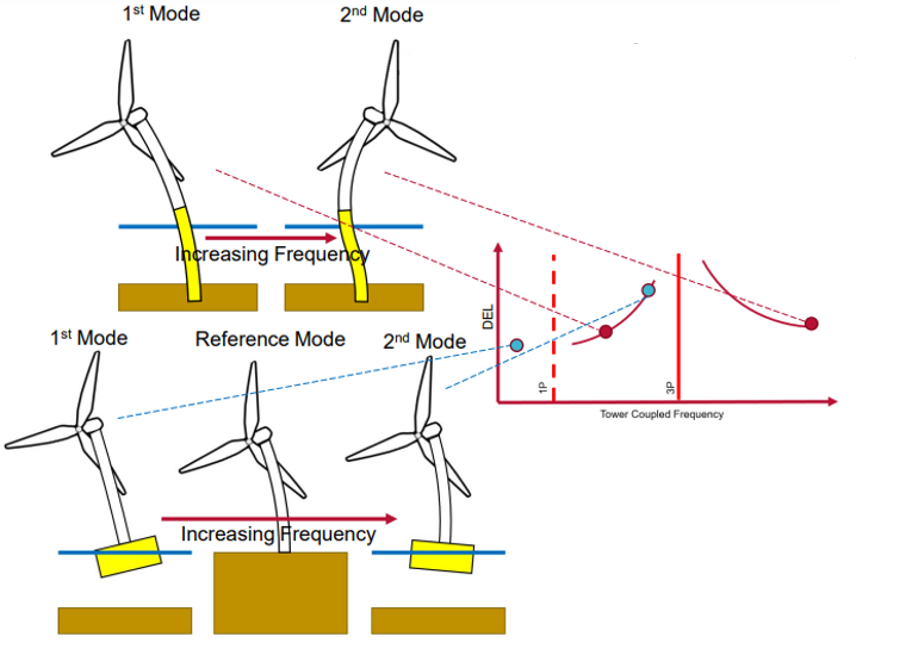
\includegraphics[width=0.7\linewidth]{Graphics/1P3PandEigenFloater.png}
	\caption{Illustration of the 1st and 2nd tower mode of both fixed-bottom and floater turbines. With floating structure the 1st mode is shiften down way past the 1P frequency}
	\label{fig:eigen_and_1p3p}
\end{figure}





